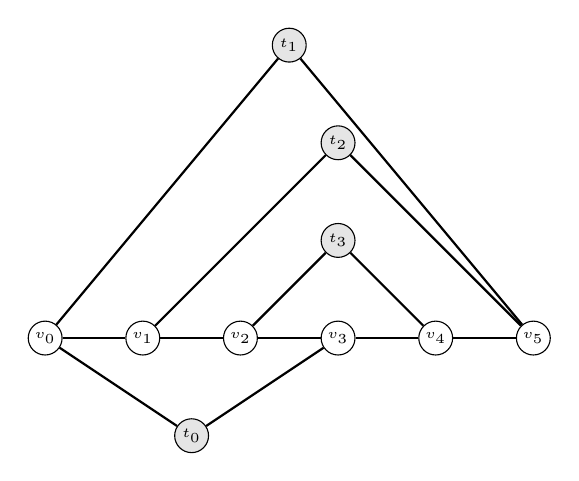
\begin{tikzpicture}[x=0.62cm, y=0.62cm, vtx/.style={circle,draw,inner sep=0.6pt,minimum size=4.3mm,font=\tiny}]
\node[vtx,fill=black!10] (t0) at (3,-2) {$t_{0}$};
\node[vtx,fill=black!10] (t1) at (5,6) {$t_{1}$};
\node[vtx,fill=black!10] (t2) at (6,4) {$t_{2}$};
\node[vtx,fill=black!10] (t3) at (6,2) {$t_{3}$};
\node[vtx] (v0) at (0,0) {$v_{0}$};
\node[vtx] (v1) at (2,0) {$v_{1}$};
\node[vtx] (v2) at (4,0) {$v_{2}$};
\node[vtx] (v3) at (6,0) {$v_{3}$};
\node[vtx] (v4) at (8,0) {$v_{4}$};
\node[vtx] (v5) at (10,0) {$v_{5}$};
\draw[thick] (v0) -- (t0);
\draw[thick] (v0) -- (t1);
\draw[thick] (v0) -- (v1);
\draw[thick] (t0) -- (v3);
\draw[thick] (t1) -- (v5);
\draw[thick] (v1) -- (t2);
\draw[thick] (v1) -- (v2);
\draw[thick] (t2) -- (v5);
\draw[thick] (v2) -- (t3);
\draw[thick] (v2) -- (v3);
\draw[thick] (t3) -- (v4);
\draw[thick] (v3) -- (v4);
\draw[thick] (v4) -- (v5);
\end{tikzpicture}
